\documentclass{article}
\usepackage{blindtext}
\usepackage[a4paper, total={6in, 9.4in}]{geometry}

\usepackage{wrapfig}
\usepackage{graphicx}
\usepackage{mathtext}
\usepackage{amsmath}
\usepackage{siunitx} % Required for alignment
\usepackage{subfigure}
\usepackage{multirow}
\usepackage{rotating}
\usepackage{afterpage}
\usepackage[T1,T2A]{fontenc}
\usepackage[russian]{babel}
\usepackage{caption}
\usepackage[arrowdel]{physics}
\usepackage{booktabs}

\graphicspath{{pictures/}}

\title{\begin{center}Лабораторная работа №3.2.8\end{center}
Релаксационные колебания}
\author{Гёлецян А.Г.}
\date{\today}

\begin{document}

\pagenumbering{gobble}
\maketitle
\newpage
\pagenumbering{arabic}

\textbf{Цель работы:} Изучение вольт-амперной характеристики нормального тлеющего
разряда; исследование релаксационного генератора на стабилитроне

\section{Теоретическая часть}

\begin{figure}[h]
    \center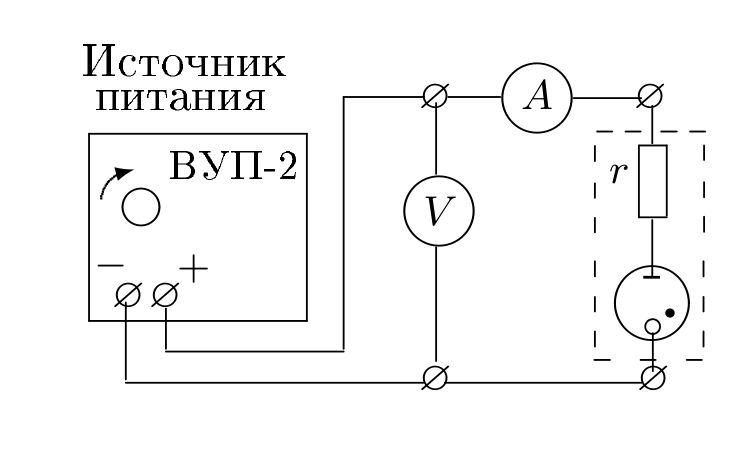
\includegraphics[width = 0.6\linewidth]{ust1.png}
    \caption{Схема установки для изучения характеристик стабилитрона}
\end{figure}
\begin{figure}[h]
    \center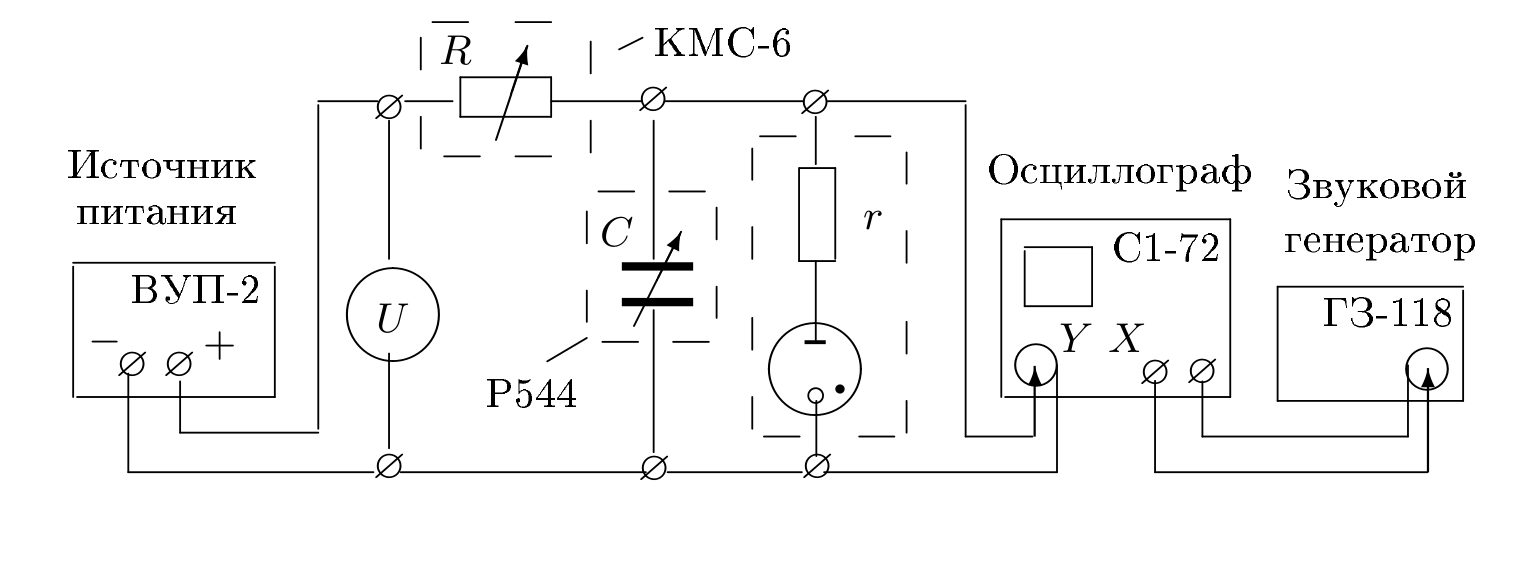
\includegraphics[width = 0.6\linewidth]{ust2.png}
    \caption{Схема установки для исследования релаксационных колебаний}
\end{figure}

Колебательные системы, как правило, имеют два накопителя энергии, между которыми
происходит её перекачка. В контуре, содержащем конденсатор и катушку индуктивности,
электрическая энергия переходит в магнитную и обратно.

Встречается, однако, колебательные системы, содержащие всего один накопитель энергии.
Рассмотрим в качестве примера электрическую цепь, содержащую конденсатор и 
сопротивление без самоиндукции. Разряд конденсатора через сопротивление представляет
собой апериодический процесс. Разряду, однако, можно придать периодический характер,
возобновляя заряд конденсатора через постоянные промежутки времени. Колебания в этом
случае являются совокупностью двух апериодических процессов --- процесса зарядки
конденсатора и процесса его разрядки.

\begin{figure}[h]
    \center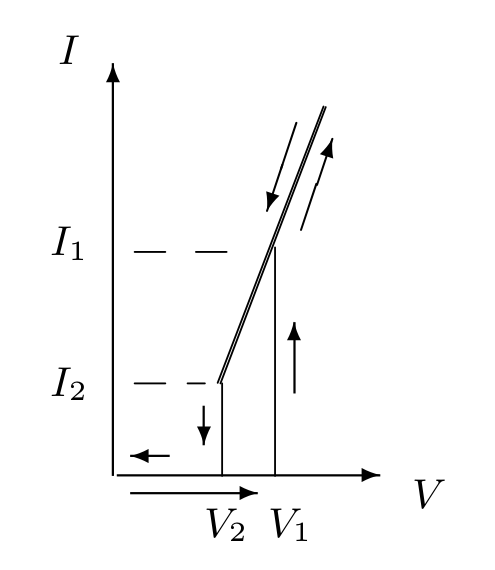
\includegraphics[width = 0.3\linewidth]{va.png}
    \caption{Вольт-амперная характеристика стабилитрона с поледовательно включённым резистором}
\end{figure}
В нашей установке роль <<ключа>>, обеспечивающего попеременную зарядку и разрядку
конденсатора, играет газоразрядный диод. Зависимость тока от напряжения для
газоразрядной лампы не подчиняется закону Ома и характеризуется рядом особенностей.
При малых напряжениях лампа практически не пропускает тока. Ток в лампе возникает
только в том случае, если разность потенциалов на её электродах достигает напряжения
зажигания $V_1 = V_\text{заж}$. При этом скачком устанавливается конечная сила тока
$I_1$ --- в лампе возникает нормальный тлеющий разряд. При дальнейшем незначительном
увеличении напряжения сила тока заметно возрастает по закону, близкому к линейному.
Нормальный тлеющий разряд --- стабилизатор напряжения, отсюда второе название лампы
--- стабиловольт.

Если начать уменьшать напряжение на горящей лампе, то при напряжении, равном
$V_\text{заж}$, лампа ещё не гаснет, а сила тока продолжает уменьшаться. Лампа перестаёт
пропускать ток лишь при напряжении гашения $V_2 = V_\text{гаш}$, которое обычно
существенно меньше $V_\text{заж}$. Сила тока при этом скачком падает от значения
$I_2 (I_2 < I_1)$ до нуля.

Изображённая выше вольт-амперная характеристика несколько идеализированна. У реальной
лампы зависимость $I(V)$ не вполне линейна. При $V > V_\text{заж}$ графики,
соответствующие возрастанию и убыванию напряжения, не всегда совпадают. Эти отличия,
впрочем, носят второстепенный характер и для нашей задачи несущественны.

\begin{figure}[h]
    \center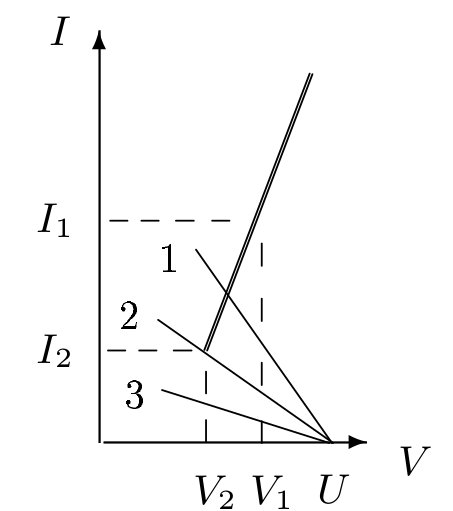
\includegraphics[width = 0.3\linewidth]{r.png}
    \caption{Режимы работы релаксационного генератора}
\end{figure}
Рассмотрим схему релаксационного генератора. Пусть напряжение батареи $U$ больше
напряжения зажигания $V_1$. В обозначениях, принятых на схеме, справедливо уравнение

\begin{equation*}
    I_C + I(V) = \frac{U - V}{R},
\end{equation*}

или 

\begin{equation*}
		C \frac{dV}{dt} + I(V) = \frac{U - V}{R}.
\end{equation*}

В стационарном режиме работы, когда напряжение $V$ yа конденсаторе постоянно и
$dV / dt = 0$, ток через лампу равен
\begin{equation*}
		I_\text{ст} = \frac{U - V}{R}.
\end{equation*}
Это равенство представлено выше графически.

При разных $R$ графики имеют вид прямых, пересекающихся в точке $V = U, I = 0$. Область,
где эти нагрузочные прямые пересекают вольт-амперную характеристику лампы, соответствует
стационарному режиму --- при малых $R$ (прямая 1) лампа горит постоянно, колебания
отсутствуют. Прямая 2, проходящая через точку $(I_2, V_2)$, соответствует критическому
сопротивлению 
\begin{equation*}
	R_\text{кр} = \frac{U - V_2}{I_2}.
\end{equation*}
При сопротивлении $R > R_\text{кр}$ нагрузочная прямая 3 не пересекает характеристику
лампы, поэтому стационарный режим невозможен. В этом случае в системе устанавливаются
колебания.

Рассмотрим, как происходит колебательный процесс. Пусть  вначале опыта ключ $K$
разомкнут и $V = 0$. Замкнём ключ. Конденсатор $C$ начинает заряжаться через
сопротивление $R$, напряжение на нём увеличивается. Как только оно достигнет
напряжения зажигания $V_\text{заж}$, лампа начинает проводить ток, причём прохождение
тока сопровождается разрядкой конденсатора. В самом деле, батарея $U$, подключённая
через большое сопротивление $R$, не может поддерживать необходимую для горения лампы
величину тока. Во время горения лампы конденсатор разряжается, и когда напряжение на
нём достигнет потенциала гашения, лампа перестанет проводить ток, а конденсатор вновь
начнёт заряжаться. Возникают релаксационные колебания с амплитудой, равной $(V_1 - V_2)$.

\begin{figure}[h]
    \center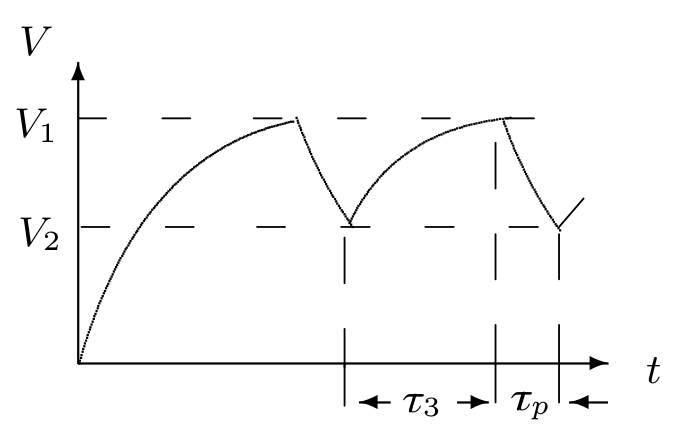
\includegraphics[width = 0.4\linewidth]{kol.png}
    \caption{Осциллограмма релаксационных колебаний}
\end{figure}
Рассчитаем период колебаний. Полное время одного периода колебаний $T$ состоит из суммы
времени зарядки $\tau_\text{з}$ и времени разрядки $\tau_\text{р}$, но если
сопротивление $R$ существенно превосходит сопротивление зажжённой лампы,
то $\tau_\text{з} \gg \tau_\text{р}$ и $T \approx \tau_\text{з}$. Во время зарядки
конденсатора лампа не горит $(I(V) = 0)$, и уравнение приобретает вид
\begin{equation*}
	RC \frac{dV}{dt} = U - V.
\end{equation*}
Будем отсчитывать время с момента гашения лампы, так что $V = V_2$ при $t = 0$. Решив
это уравнение, найдём
\begin{equation*}
	V = U - (U - V_2) e^{-t / RC}.
\end{equation*}
В момент зажигания $t = \tau_\text{з}, V = V_1$, поэтому
\begin{equation*}
	V_1 = U - (U - V_2) e^{\tau_\text{з} / RC}.
\end{equation*}
Из этих двух уравнений нетрудно найти период колебаний:
\begin{equation*}
	T \approx \tau_\text{з} = RC \ln \frac{U - V_2}{U - V_1}.
\end{equation*}

\newpage
\section{Ход работы}
\subsection{Вольт-амперная характеристика}
Для начала измерим вольт--амперную характеристику стабилитрона
\begin{figure}[h]
    \center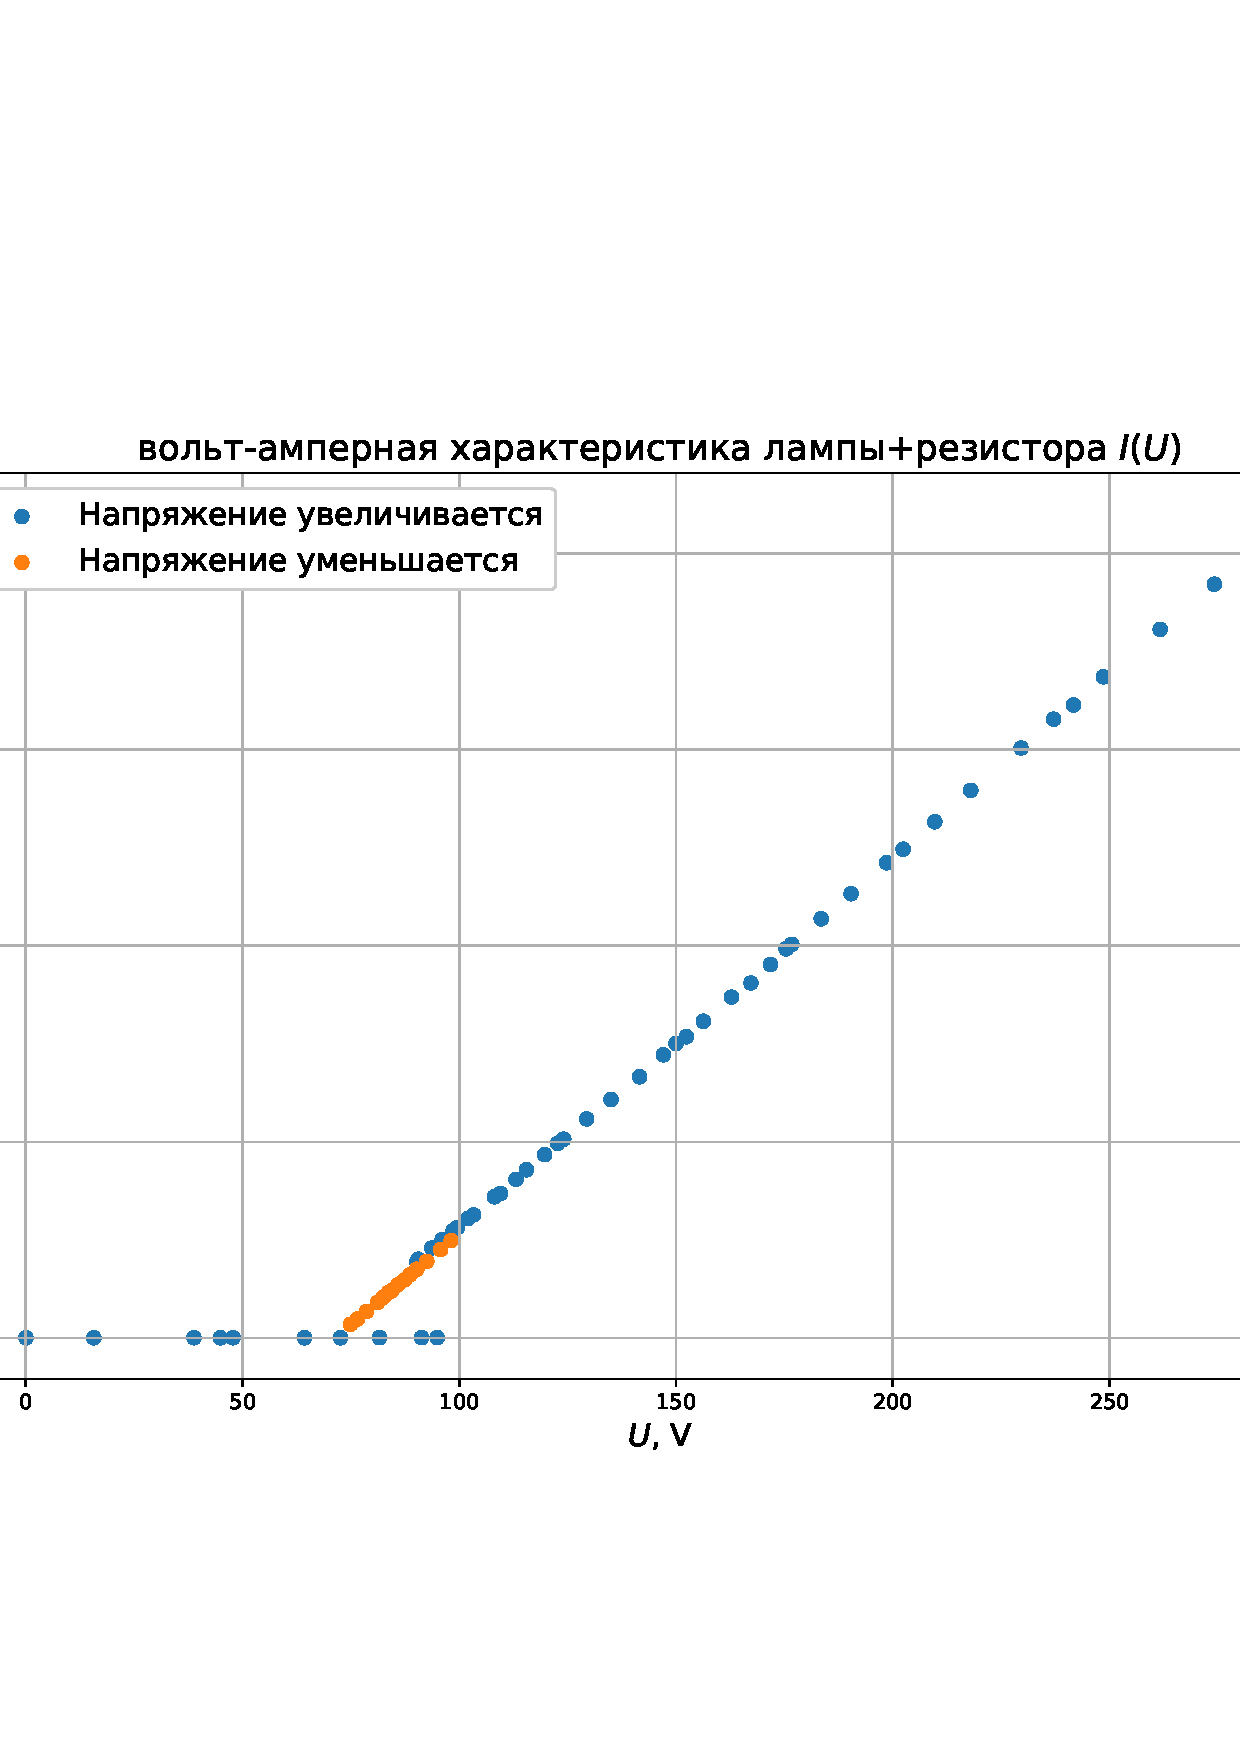
\includegraphics[width = 0.80\linewidth]{R_IU}
    \caption{ВАХ сборки резистор-стабилитрон}
\end{figure}

\begin{figure}[h]
    \center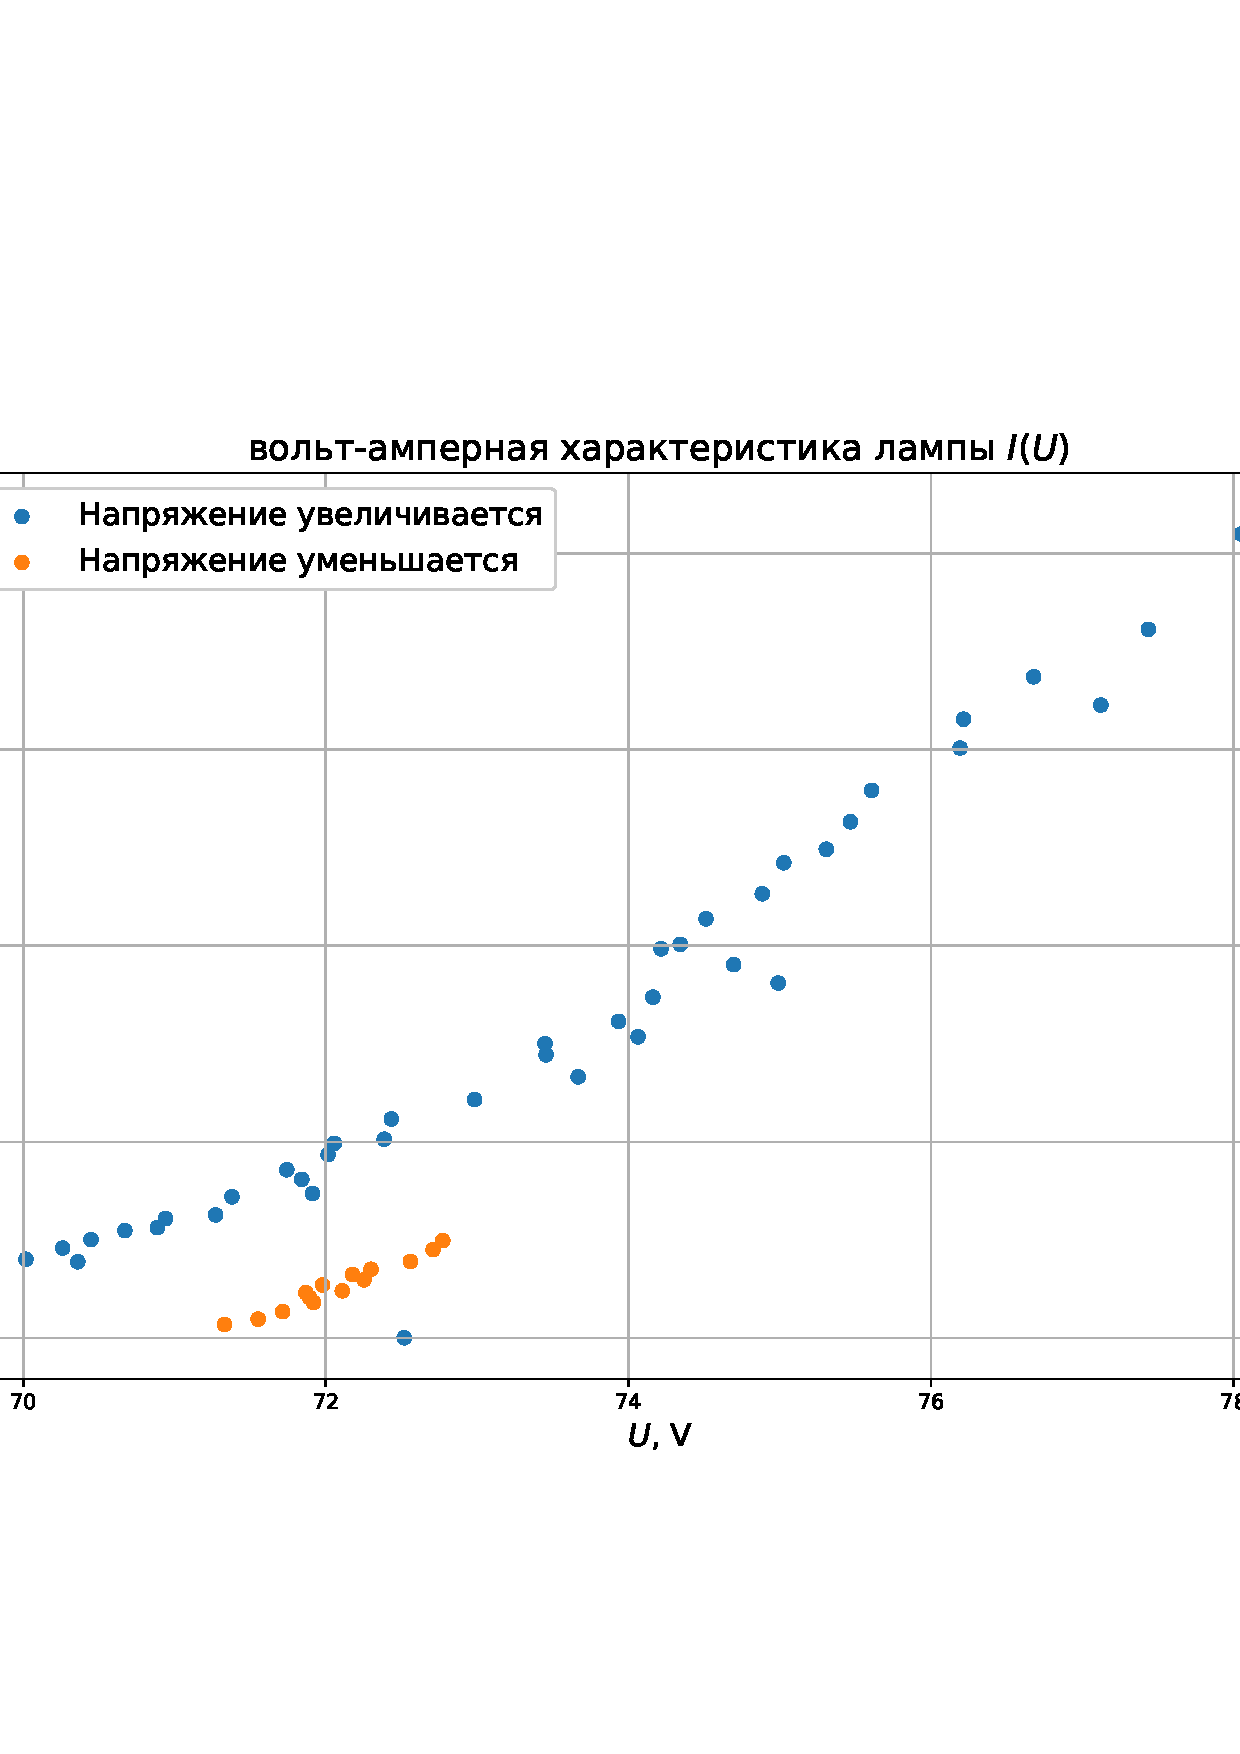
\includegraphics[width = 0.80\linewidth]{stab_IU}
    \caption{ВАХ стабилитрона}
\end{figure}

Как видим, ВАХ расщипляется на 2 линии в зависимости от направления изменения
напряжения. Так же были измерены потенциалы зажигания и гашения.
\begin{align*}
    V_1 &= (95.0 \pm 0.5)В\\
    V_2 &= (74.2 \pm 0.2)В
\end{align*}

\subsection{Релаксационные колебания}

Выставляя напряжение $U=118В$, емкость $C=50нф$, уменьшаем сопротивление до тех пор,
пока не перейдем в стационарный режим работы. Таким образом находим
$R_{кр}\approx170к\Omega$.

Выставляем напряжение $U=115В$, сопротивление $R=500к\Omega$, и изучаем зависимость
периода от емкости $C$.

\begin{figure}[h]
    \center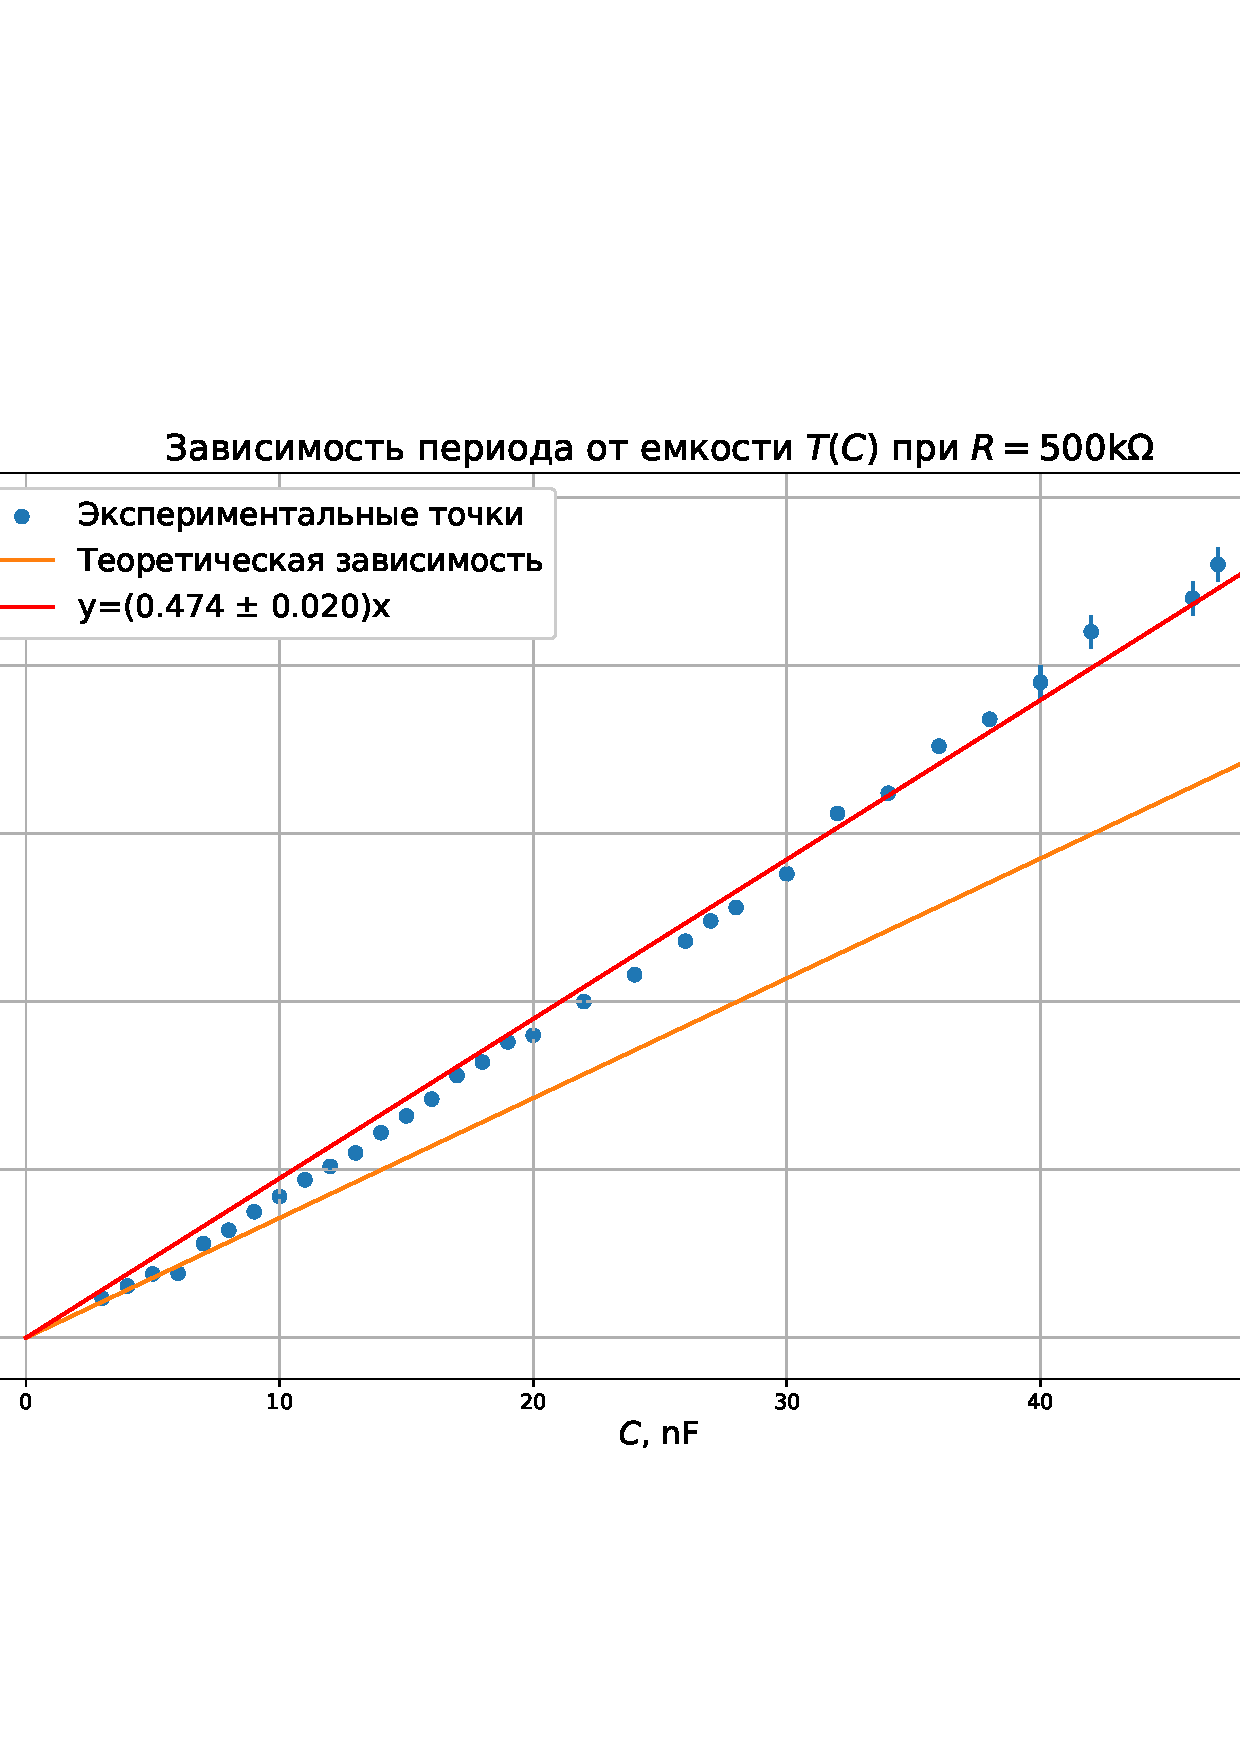
\includegraphics[width = 1\linewidth]{T_C}
    \caption{График зависимости периода от емкости}
\end{figure}

Как видим, зависимость похоже на линейную, но значения, расчитанные по теоретической
формуле, систематически находятся ниже измеренных напряжений. Если предположить, что
это связано только с изменением потенциала гашения в динамическом режиме работы, то
из экспериментальных данных можем получить динамический потенциал гашения
\begin{equation*}
    V_{2, дин}^{R=\text{const}} = (63.4 \pm 2.0) В
\end{equation*}

Проделав похожие измерения, фиксировав $C$ и меняя $R$ получим другую зависимость. Из
тех же самых предположений посчитаем динамический потенциал гашения и в этом случае.
\begin{equation*}
    V_{2, дин}^{C=\text{const}} = (59.1 \pm 1.9) В
\end{equation*}

\newpage
\begin{figure}[h]
    \center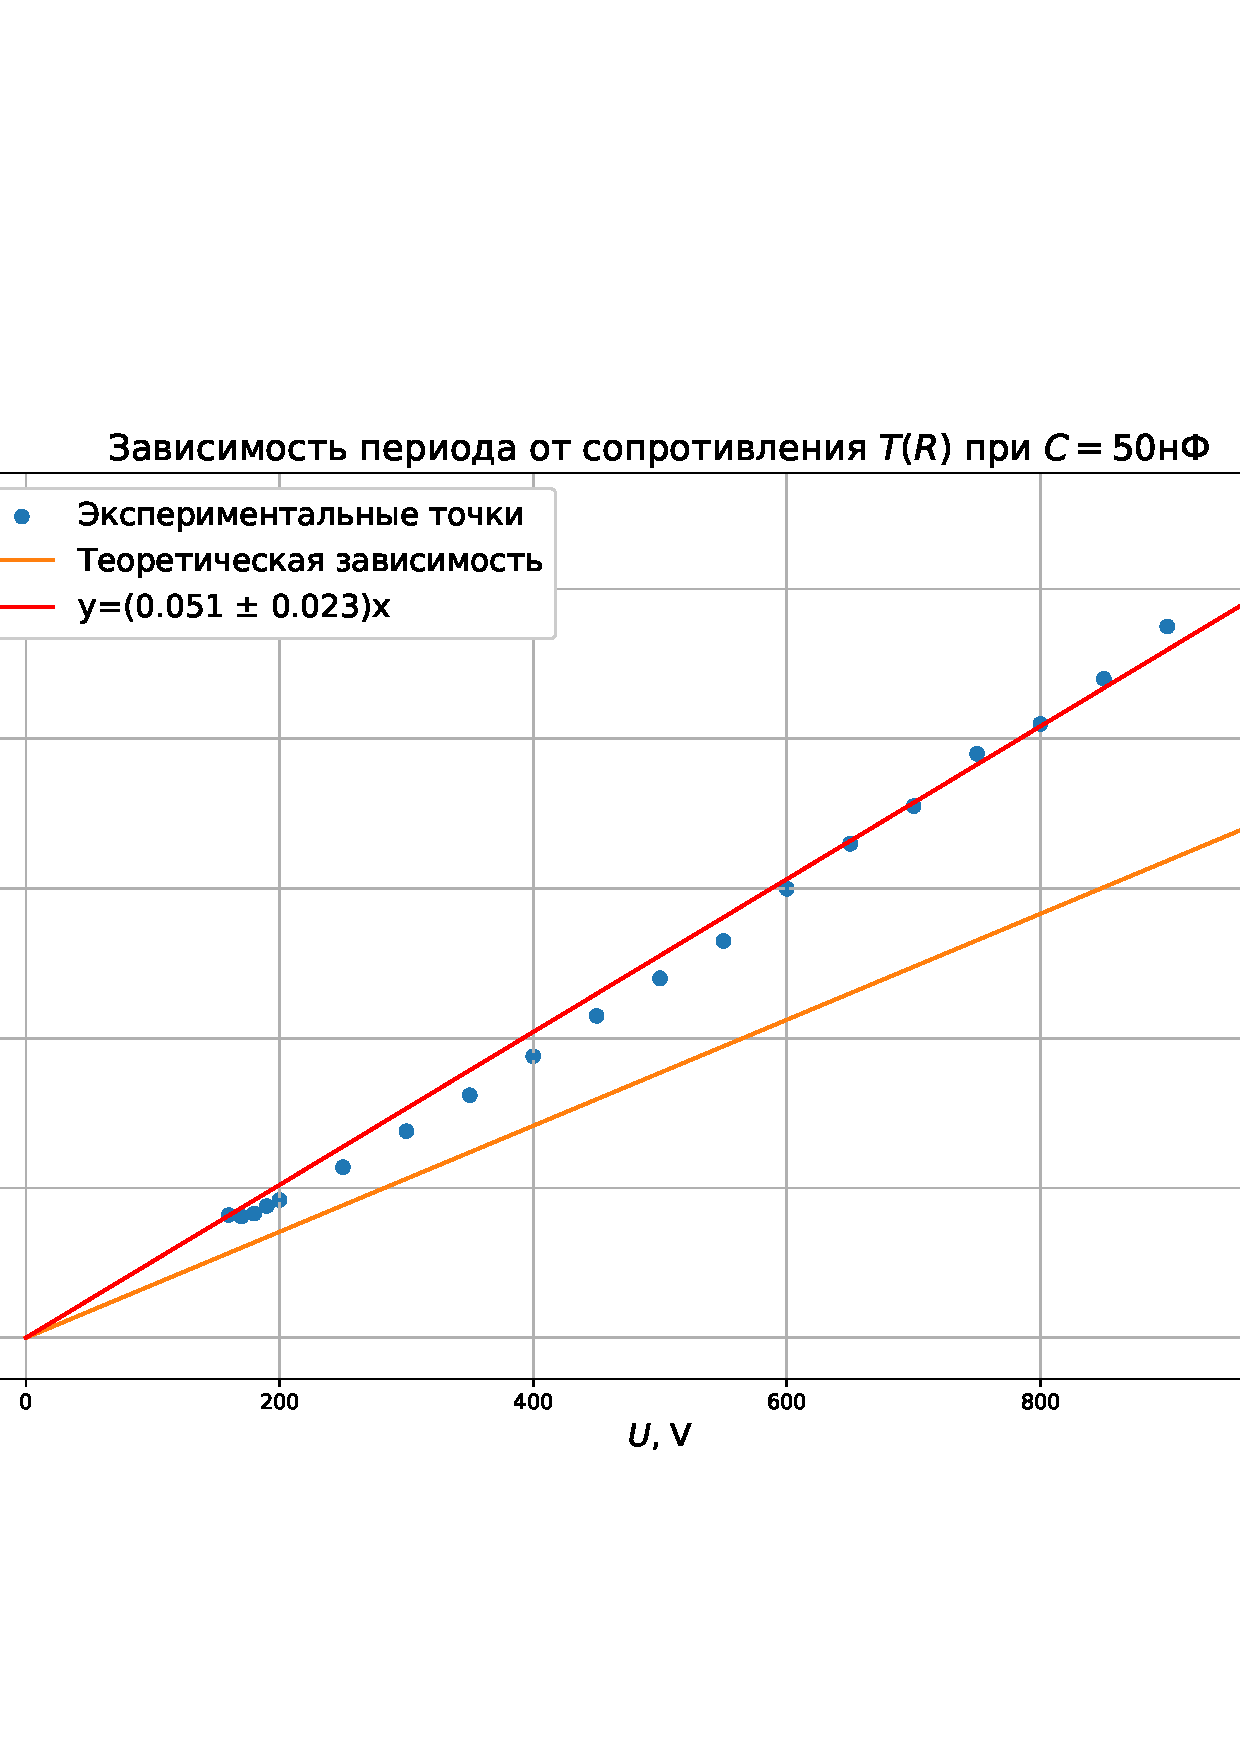
\includegraphics[width = \linewidth]{T_R}
    \caption{График зависимости периода от сопротивления}
\end{figure}
\begin{figure}[h]
    \center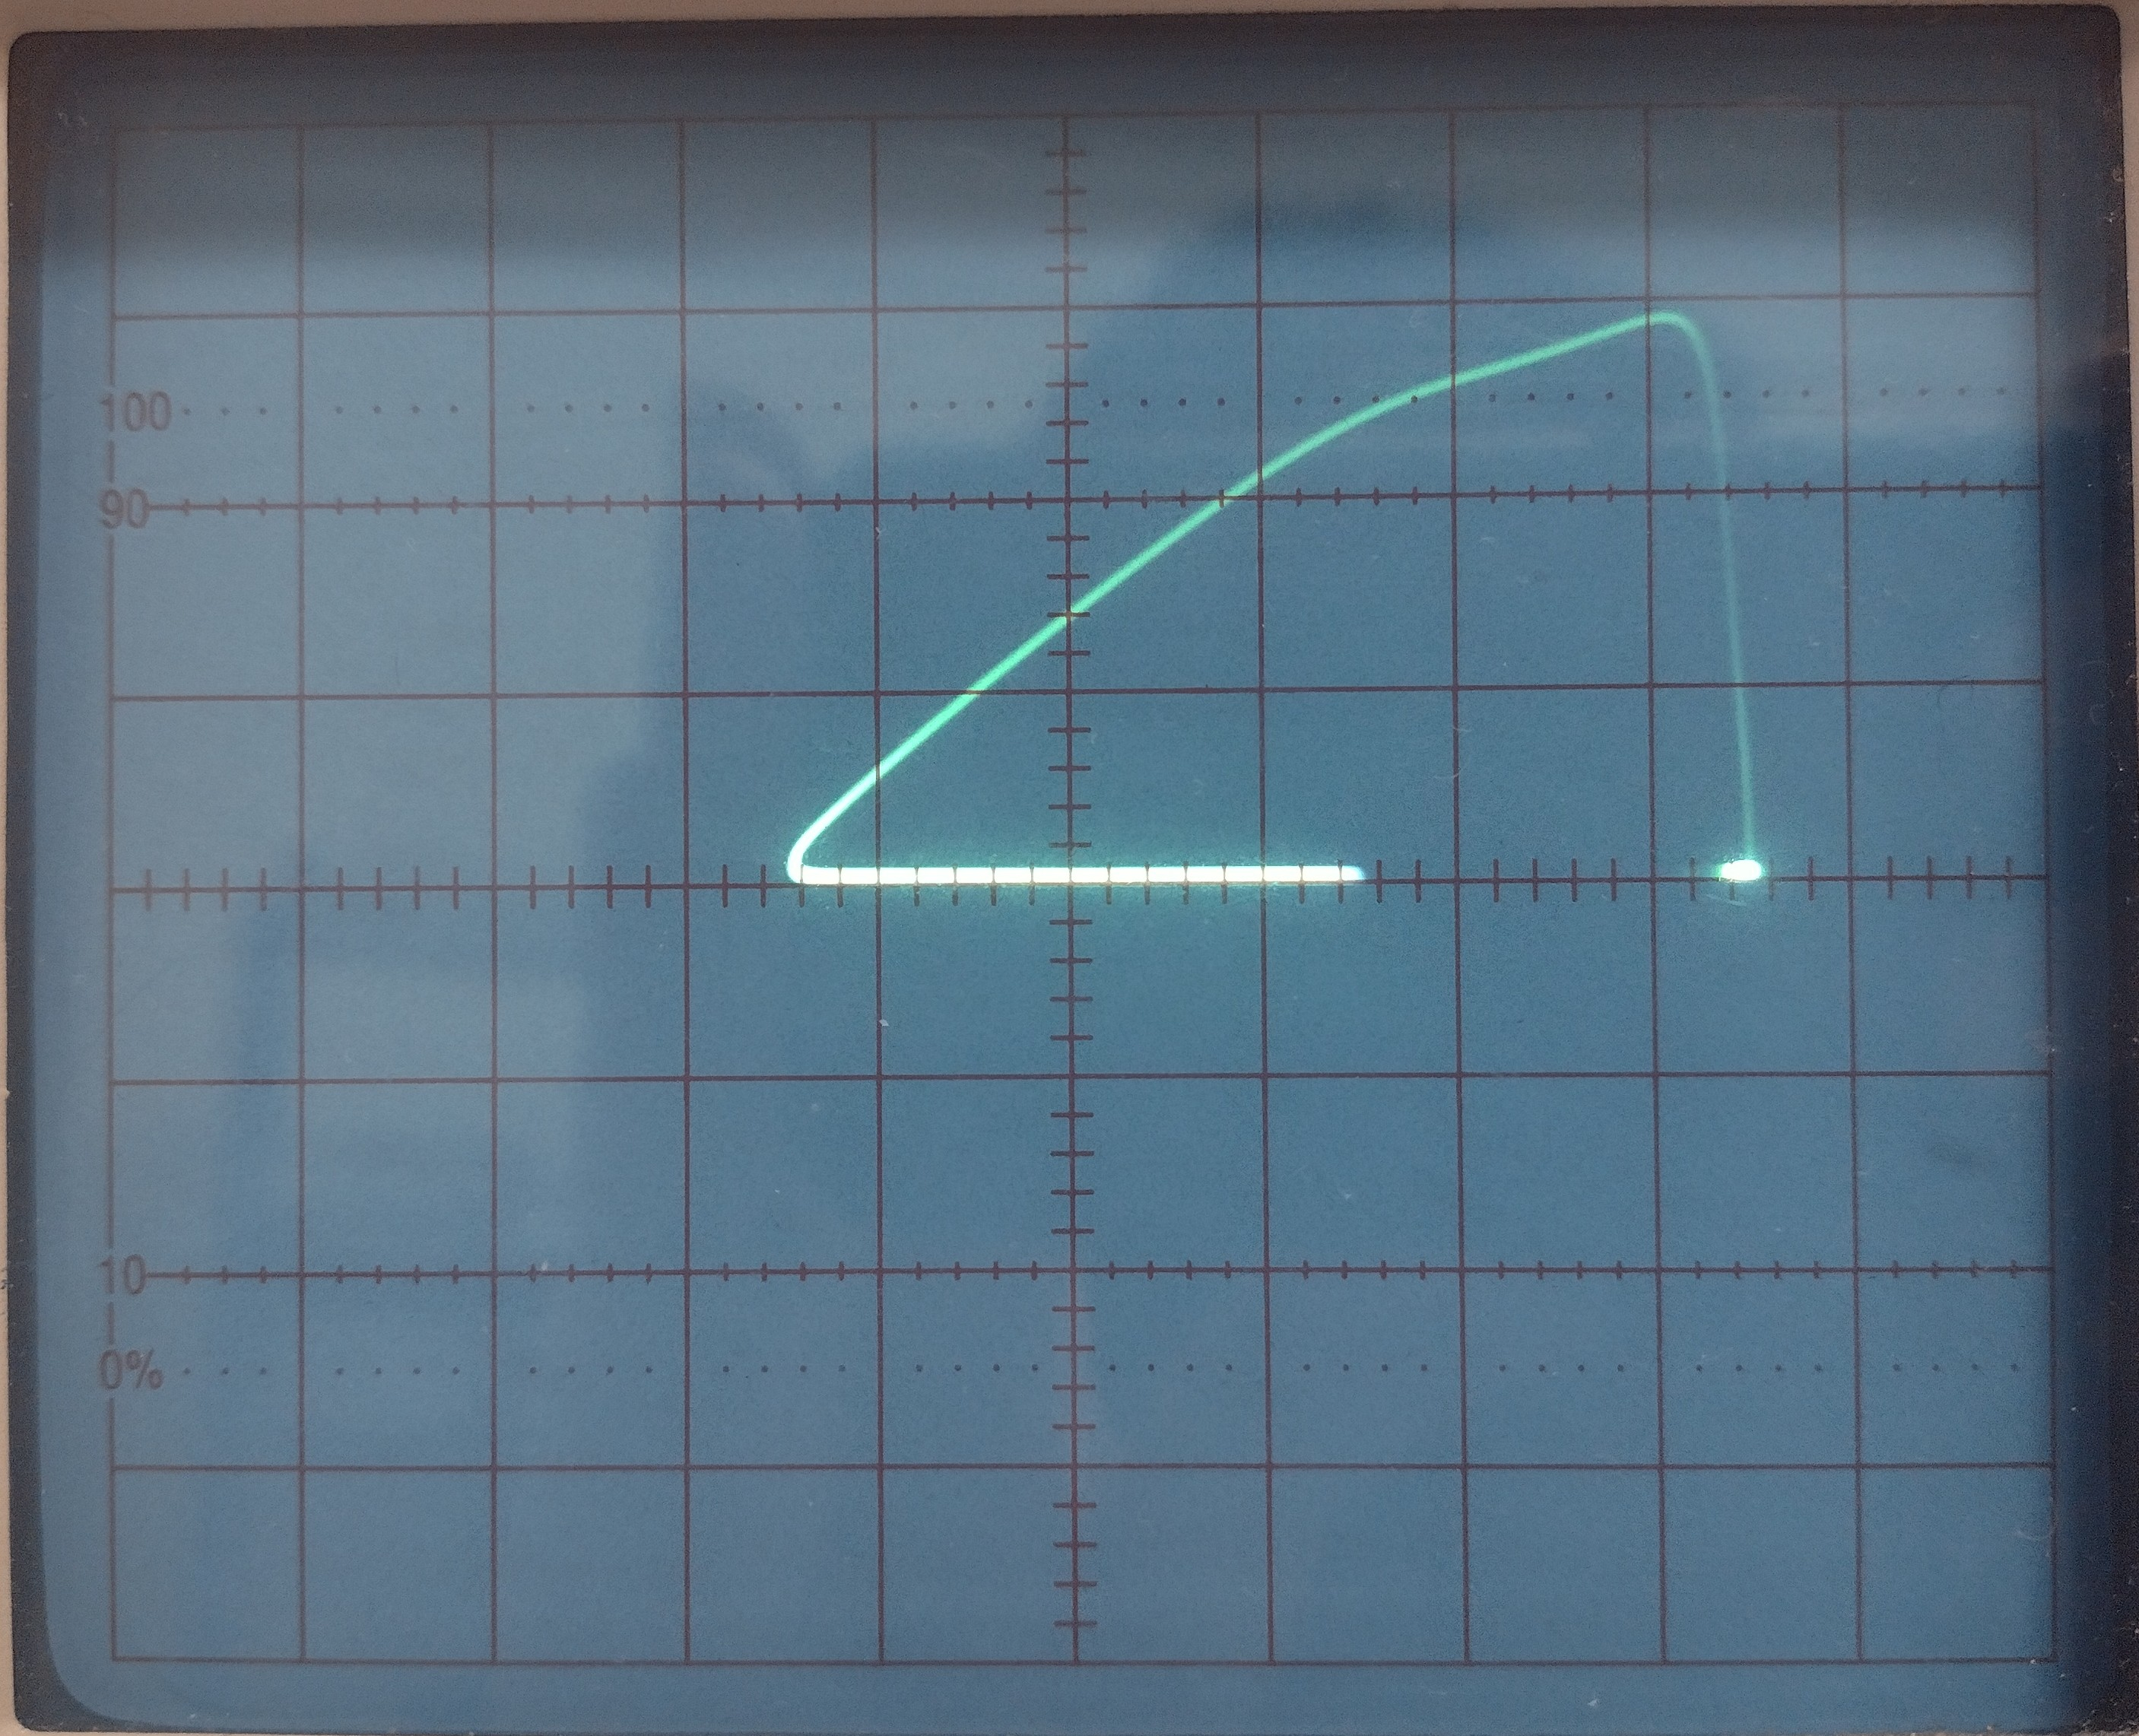
\includegraphics[width = 0.49\linewidth]{phase_diagram}
    \caption{Фазовая диаграма $V-I$ при $U=116.0В$, $C=50нф$, $R=900к\Omega$}
\end{figure}

\newpage
\begin{figure}[h]
    \center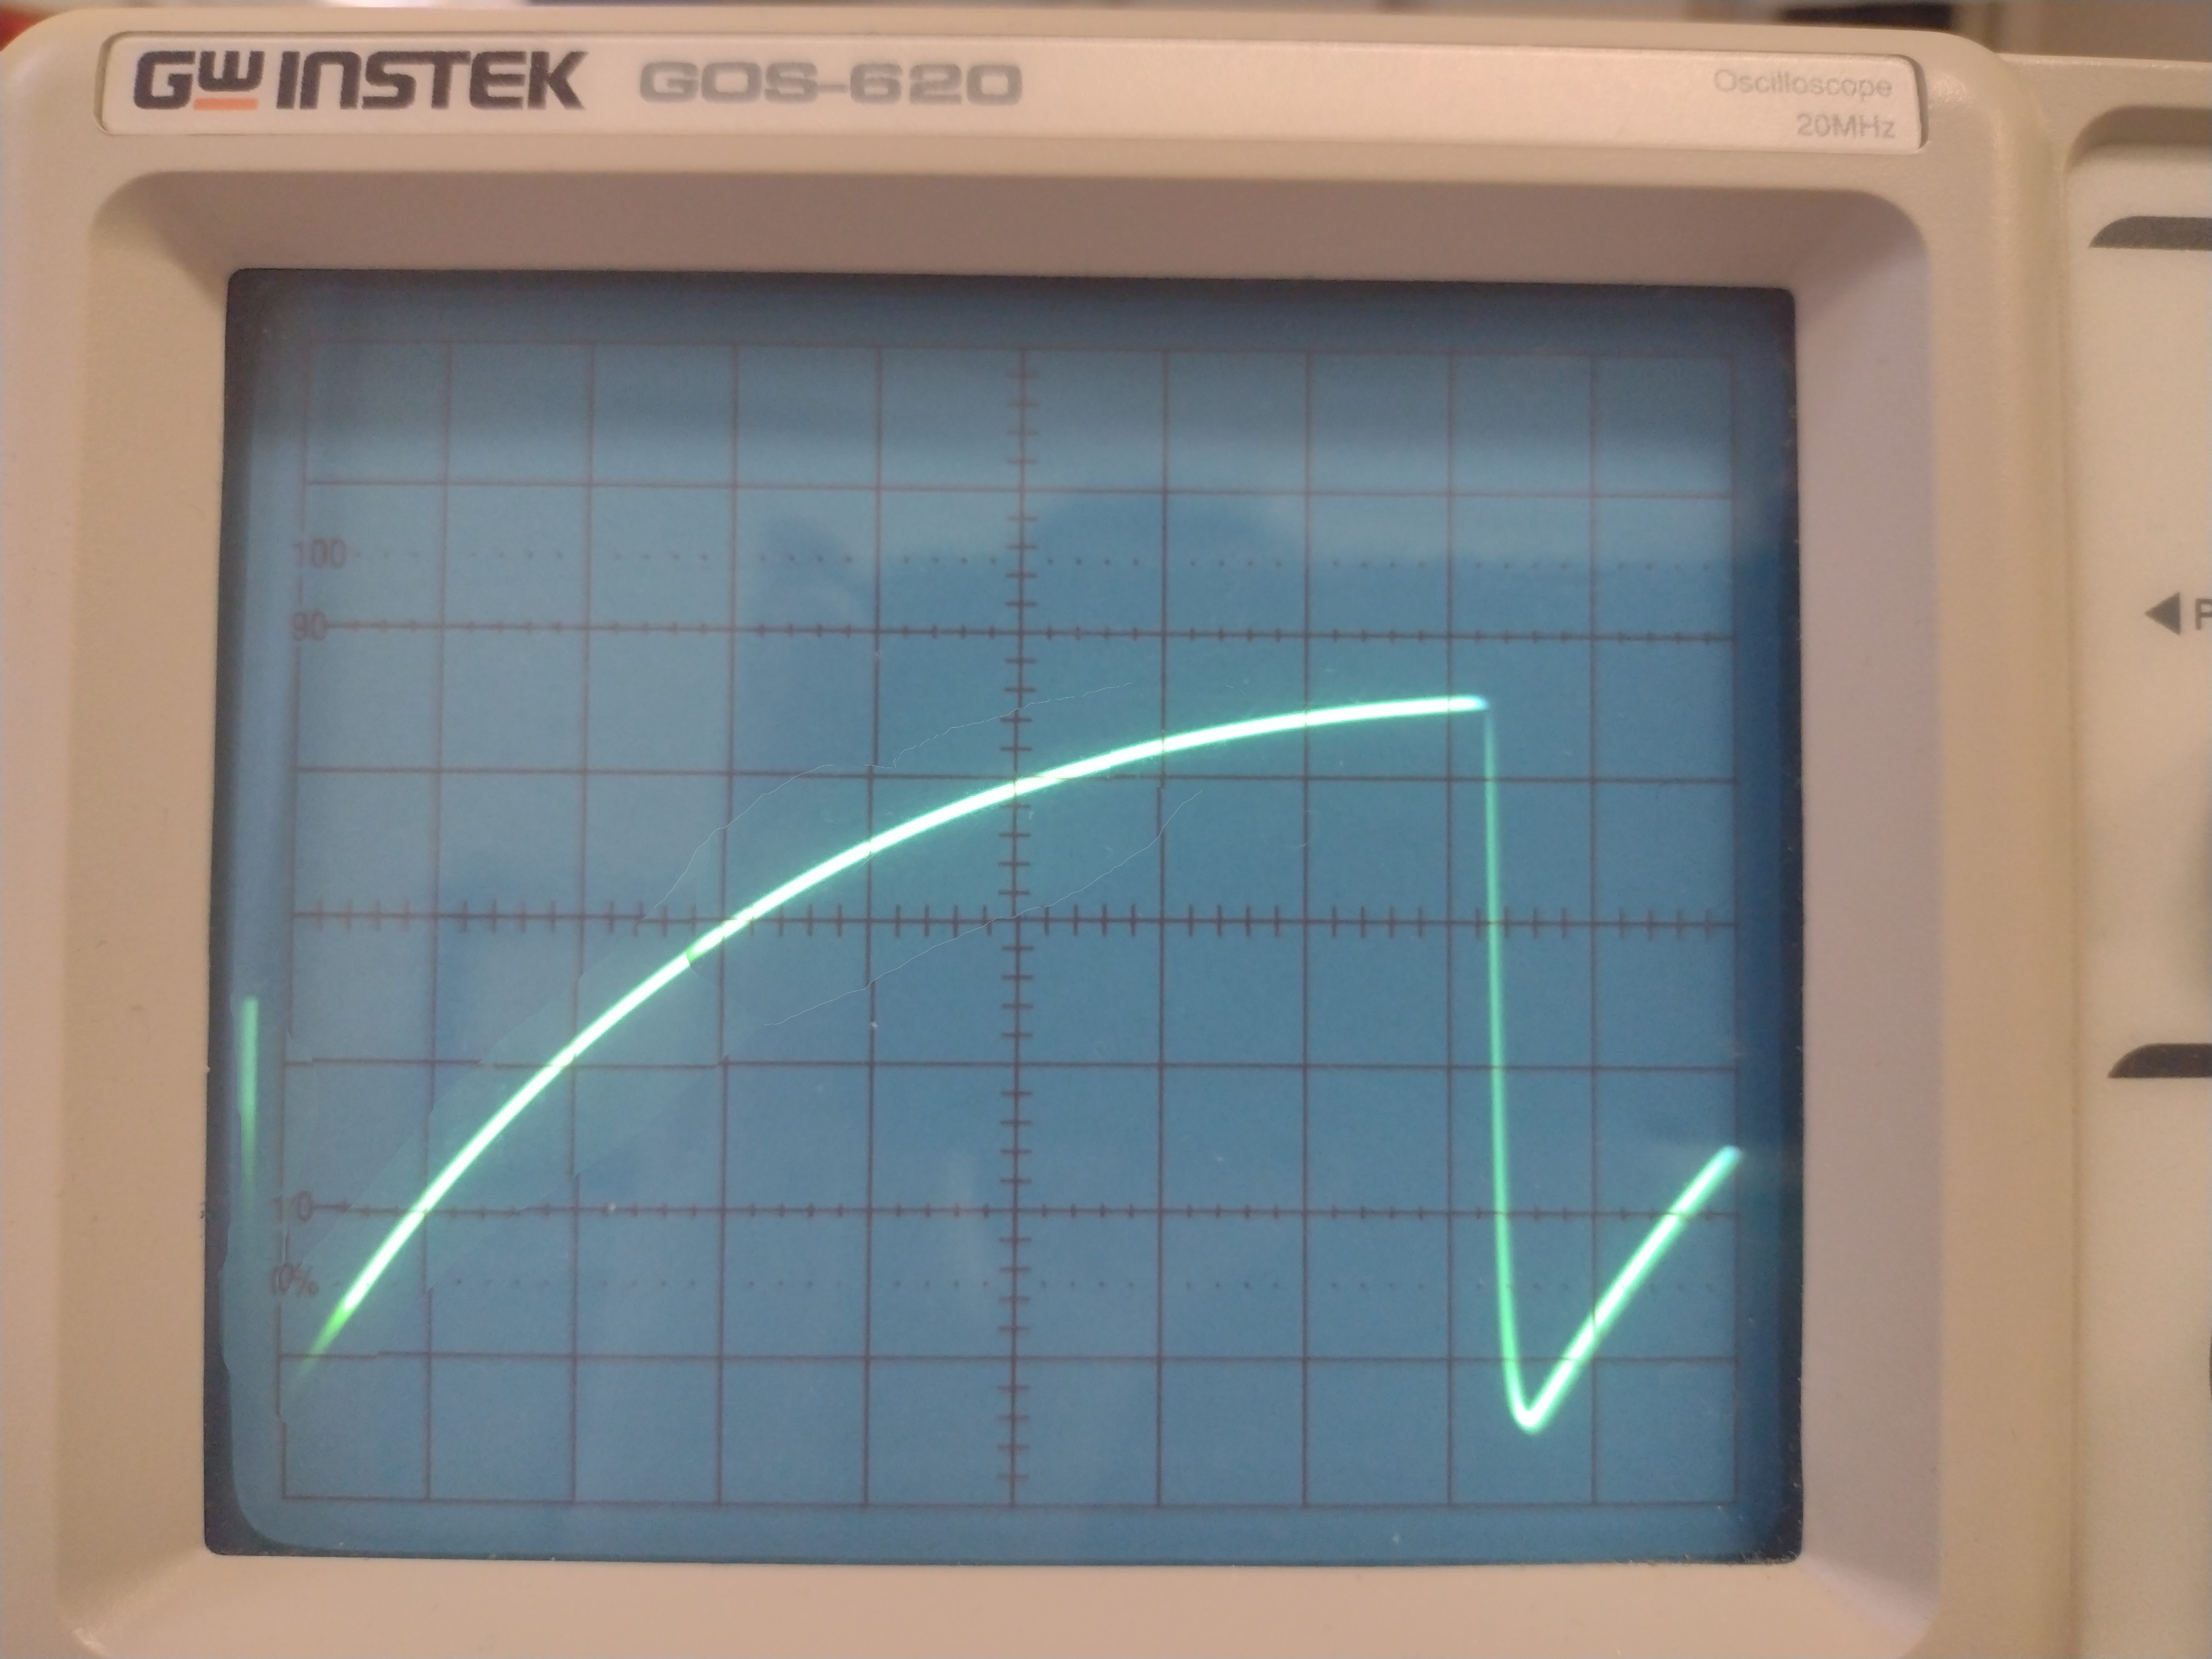
\includegraphics[width = 0.6\linewidth]{oscillogram/merged.jpg}
    \caption{Осциллограмма автоколебаний}
\end{figure}

\section{Выводы}
Из ВАХ стабилитрона можем сделать вывод, что стабилитрон работает, и может
стабилизировать напряжение. Из результатов видно, что динамический потенциал гашения
значительно ($\sim10-14 В$) меньше статического напряжения гашения. В пределах применения
теоретической модели наблюдается прямопропорциональная зависимость периода от
сопротивления и емкости.
\end{document}

